\documentclass[12pt]{article}
\usepackage[margin=1in]{geometry} 
\usepackage{amsmath}
\usepackage{tcolorbox}
\usepackage{amssymb}
\usepackage{amsthm}
\usepackage{lastpage}
\usepackage{fancyhdr}
\usepackage{accents}
\pagestyle{fancy}
\setlength{\headheight}{40pt}


\newenvironment{solution}
  {\renewcommand\qedsymbol{$\blacksquare$}
  \begin{proof}[Solution]}
  {\end{proof}}
\renewcommand\qedsymbol{$\blacksquare$}

\newcommand{\ubar}[1]{\underaccent{\bar}{#1}} % add packages, settings, and declarations in settings.tex
\usepackage{url}
\begin{document}

\lhead{Prof. C.E. Tsourakakis} 
\rhead{CS365 Spring '22 \\ Foundations of Data Science \\ Assignment 1} 
\cfoot{\thepage\ of \pageref{LastPage}}


\section*{Instructions}
\framebox{%
	\begin{minipage}{0.9\linewidth}
		\begin{itemize}
			\item The homework is due on \underline{{\bf Friday 2/4 at 5pm ET}}.  
			\item There are 4 problems, and 3 pages in total.
			\item No extension will be provided, unless for serious documented reasons.
			\item {\bf Start early!}
			\item Study the material taught in class, and feel free to do so in small groups, but the solutions should be a product of your own work. 
			%\item For any given problem, the points per sub-question are equally distributed {\it unless otherwise told}. For example, Problems 2.1, 2.2, 2.3  are worth $\frac{30}{3}=10$ points each. Problem 2.2(i) and (ii) similarly are worth 5 points each. However, Problem 3 has unequal distribution of points that is explicitly given. 
			\item This  is not a multiple choice homework;   reasoning, and mathematical proofs are required before giving your final answer.
			\item The code necessary to generate the plots in Problems 2.1, and 3.1,  should be included  in the PDF of your solutions; see \url{https://www.overleaf.com/learn/latex/Code_listing} for several ways this can be done in LaTeX, that is the recommended language to typeset your solutions.
		\end{itemize}
\end{minipage}}


\section{Is there a path from $s$ to $t$? [15 points]}  
 \begin{figure*}[!ht]
	\centering
	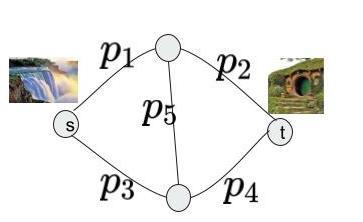
\includegraphics[width=0.5\textwidth]{pipes}
	\caption{\label{fig:pipes} How likely is water to reach $t$ from $s$?}
\end{figure*}

Consider the network shown in Figure~\ref{fig:pipes}. Recall that $p_i$ is the probability pipe $i$ breaks down, and that pipes break down independently. 



\begin{tcolorbox}
	\begin{enumerate}
		\item What is the probability water can go from the water source $s$ to the destination village $t$? Explain your answer. You do not need to simplify it algebraically.
	%	\item Let $p_i=10^{-3}$ for $i=1,..,5$. Compare your answer from (1) to Benforroni's inequalities for $m=1,2$.  
	\end{enumerate}
\end{tcolorbox}


\newpage 

\section{PIN Cracker [30 Points] } 
John has a cell phone with a PIN that consists of 4 digits (0-9). Unfortunately John totally forgot his PIN, but at least he can try PIN numbers as many times as he wants to without blocking the device.  He applies the following two strategies\footnote{In reality, there exist better strategies to break a PIN \url{https://www.popsci.com/technology/article/2012-09/infographic-day-fastest-way-crack-4-digit-pin-number/}, but let's assume we employ only naive strategies here.}:

\begin{itemize}
    \item[($s_1$)] He tries a valid PIN uniformly at random each hour, till he enters the right one.
    \item[($s_2$)] He keeps track of the unsuccessful attempts, and chooses a PIN uniformly at random from the PIN numbers he has not tried yet. 
\end{itemize}

\begin{tcolorbox}
\begin{enumerate}
    \item  {\bf [10 points] } Write code that simulates strategies $s_1$ and $s_2$. You may assume that the correct PIN is 2022 in your code. Simulate each strategy 100, 200, 300, ..., 1\,000 times, and report for each number of trials the average number of trials, and the standard deviation till John figures out his PIN. Present your empirical findings in two plots (one per strategy) with error bars, where the $x$-axis is the number of trials.  
    \item  Let $X_1,X_2$ be the number of trials under strategies $s_1$ and $s_2$ respectively. Compute their expectations analytically: 
    \begin{itemize}
        \item[i)]   {\bf [5 points] }$ \mathbb{E}[X_1]$.
        \item[ii)]  {\bf [5 points] } $ \mathbb{E}[X_2]$.
    \end{itemize} 


\item  {\bf [10 points] } Apply Markov's inequality to upper bound the probability $\mathbb{P}(X_i \geq 7\,000)$ for $i=1,2$.  Does Markov's inequality always provide meaningful bounds?
\end{enumerate}
\end{tcolorbox}

\newpage 

\section{Mixture of Gaussians [40 points]} 

Let $X,Y$ be two independent normal RVs, with means $\mu_x=100, \mu_y=300$ and standard deviations $\sigma_x=\sigma_y=10$. Consider the RV $U$ defined by 

$$ U = \frac{1}{2}(X+Y).$$


\noindent Alternatively,  consider the RV $Z$ that is generated as follows:

\begin{itemize}
	\item[(a)] With probability $\frac{1}{2}$ we sample $Z$ from $N(\mu=100, \sigma^2=10)$. 
	\item[(b)] With probability $\frac{1}{2}$ we sample $Z$ from $N(\mu=300, \sigma^2=10)$. 
\end{itemize}  


\begin{tcolorbox}
	\begin{enumerate}
		\item {\bf [10 points] } Simulate the sampling, and produce two histograms (one for $U$ and one for $Z$) over 10\,000 samples for each $U,Z$.    
		\item {\bf [10 points] } Compute the expected values of $U,Z$.
		\item {\bf [20 points] } Compute the variances  of $U,Z$.  
\item[] {\it Hint:} To compute the variance of $Z$, it will be helpful express $Z$ as a function of $X,Y$ and  an indicator variable {\bf I} that indicates from which of the two distributions (a),(b) the realization of $Z$ was drawn.
	%	\item Which variance is larger, and when does the equality  	$\Var{U}=\Var{Z}$ hold?
	\end{enumerate}
	
\end{tcolorbox}

\section{Gambling [15 points]} 

Suppose a casino has a finite fortune $F$  (e.g., 10.5M\$) that is willing to put on a table against you. You play the following game against the casino using a fair coin: if heads (H) appear for the first time after $k$ tosses, the game is over, and you get paid $2^k$ dollars. We agree to toss the coin $n$ times  or until it shows up heads, whatever happens first.   

\begin{tcolorbox}
\begin{enumerate}
   % \item What is the expected value of the bet?
    %\item[] {\bf Hint:} Consider four cases, based on whether $F$ is a power of 2, or not, and if $F> 2^n$ or not.
    \item How much money would you be willing to put on this bet if $F$=10\,500\,000\$, $n=30$? Report your answer with 4 decimal digits of accuracy.  
\end{enumerate}
 
\end{tcolorbox}


\end{document}
